\subsection{Investimento residencial nos modelos macroeconométricos}\label{RevEmpirica}

Compreendida a importância do investimento residencial para a dinâmica macroeconômica americana, faz-se necessária uma investigação dos determinantes deste gasto de acordo com a literatura econométrica e este é o objetivo desta seção. 
É importante pontuar que nos anos que procederam à crise do mercado imobiliário, verificou-se um crescente interesse nas implicações macroeconômicas do investimento residencial\footnote{Inspecionando modelos DSGE que incluem investimento residencial, \textcite{iacoviello_housing_2010} conclui que um melhor entendimento dos impactos deste gasto se faz necessária para a compreensão das flutuações macroeconômicas. Outros estudos, por sua vez, têm enfatizado o efeito riqueza sobre o consumo via valorização dos imóveis e indicam tais canais de transmissão são mais incidentes, em ordem, sobre Estados Unidos e Grã Bretanha mas mais brandos no caso francês e alemão \cites{sastre_assessment_2010}{chauvin_wealth_2010}{bassanetti_effects_2010}{arrondel_housing_2010}. 
	\textcite{alvarez_does_2010}, por sua vez, concluem que tal tipo de investimento antecede o ciclo econômico para o caso de espanhol e resultados semelhantes podem ser encontrados para França, Espanha  e Itália enquanto na Alemanha esta dinâmica é distinta \cites{ferrara_common_2010}{ferrara_cyclical_2010}.}. 

Um estudo que se sobressai é o de \textcite{poterba_tax_1984}  cuja especificação do investimento residencial depende positivamente do preço dos imóveis. 
Por mais que este trabalho seja o pioneiro ao não pressupor que a oferta de imóveis tende instantaneamente ao nível desejado, não inclui bolha de ativos.
Diante desta omissão, 
\textcite{arestis_residential_2015} estendem a contribuição de 
\textcite{poterba_tax_1984} por meio de um modelo ARDL para 17 países da OCDE. 
Dentre as conclusões, destaca-se a importância da renda disponível como principal determinante do investimento residencial para os países em questão.  A implicação deste resultado, no entanto, questionaria a possibilidade de tratar o investimento residencial enquanto um gasto autônomo e, portanto, comprometeria a análise a partir do supermultiplicador sraffiano. Este estudo, porém, conclui que tal resultado não é estatisticamente significante para o caso norte-americano em que o preço dos imóveis, bem como o acesso ao crédito são os principais determinantes desse gasto e, desse modo, reaviva a discussão para a presente investigação.


Outro estudo recente é o de \textcite{huang_is_2018} em que os autores testam ambas as hipóteses aventadas por \textcite{leamer_housing_2007} a respeito do investimento residencial (predição e causalidade). Para isso, estimam um modelo VAR estrutural (SVAR) com transformada \textit{wavelets} para os países da OCDE\footnote{
	Além de testar se a construção de novos imóveis antecipa movimentos no ciclo econômico, os autores também testam os canais de transmissão da política monetária em quatro frentes: (i) teoria neoclásica do investimento residencial; (ii) efeito-riqueza do preço dos imóveis sobre o consumo por meio de um modelo de ciclo de vida; (iii) efeito do colateral sobre o balanço patrimonial das famílias e consumo; (iv) efeito do colateral sobre o balanço patrimonial dos bancos e oferta de crédito.}.  
Os autores concluem que o investimento residencial não é um mero canal de transmissão da política monetária e que possui efeitos temporalmente distintos sobre o ciclo econômico. No curto prazo, a construção de novos imóveis tem maior capacidade preditiva enquanto o preço dos imóveis tem maior influência no longo prazo\footnote{Adicionalmente, \textcite{huang_is_2018} também concluem que a capacidade preditiva do investimento residencial é maior quanto maior a parcela deste gasto no produto.}. A razão desta distinção, argumentam, é que a transmissão da política monetária via o canal da riqueza é mais proeminente no longo prazo enquanto os canais de crédito e de colateral são mais presentes no curto prazo. Já no que diz respeito a relação causal estabelecida por \textcite{leamer_housing_2007}, afirmam que os resultados não são conclusivos para todos os países diante da heterogeneidade institucional observada\footnote{
	No entanto, os autores afirmam que para a maioria dos países do G7 o investimento residencial é ao menos capaz de amplificar o ciclo econômico.}, mas ainda é valida para os Estados Unidos\footnote{
	Apenas para ilustrar a dimensão da importância do investimento residencial para o ciclo econômico norte-americano, \textcite{huang_is_2018} utilizam este pais como critério de comparação.}.
Apesar dos resultados não conclusivos sobre as flutuações, concluem que as variáveis associadas ao investimento residencial (preço dos imóveis, taxa real de juros das hipotecas --- deflacionada por um índice geral de preços --- e \textit{spread} bancário) lideram o crescimento econômico.

Apesar de relevante, o estudo  de \textcite{huang_is_2018} reportado acima é centrado em determinantes do lado da oferta.
Uma alternativa é o de \textcite{gauger_residential_2003} em que os autores investigam os efeitos da desregulamentação das instituições depositárias ao longo da década de 80. Para tanto, estimam um VECM entre agregados monetários (M2), PIB, investimento residencial e alternam entre taxas de juros dos títulos públicos  de curto prazo e taxas de juros hipotecárias de longo prazo.
Dentre as conclusões, os autores destacam que a taxa de juros hipotecária (longo prazo) passa a contribuir cada vez mais para variância do investimento residencial:

\begin{citacao}
	\textit{The findings for the two interest rates give valuable information to evaluate results in
	other studies. Results here suggest that use of a short-term FFR and post-deregulation data
	may lead to conclusions that `interest rate shocks are much less important after
	deregulation.' The fuller slate of evidence here indicates that interest rate shocks remain
	important post-deregulation; however, now it is the long-term rate shocks that carry more
	information for housing sector movements} \cite[p.~346]{gauger_residential_2003}
\end{citacao}

As conclusões deste estudo são bastante relevantes para a presente pesquisa pelas seguintes razões: 
	(i) nível do produto é determinado --- tal como sugerido pelo supermultiplicador sraffiano --- pelo investimento residencial e ambos os gastos apresentam uma tendência comum no longo prazo e; 
	%TODO Rever resultado
	(ii) destaca a importância de mudanças institucionais para o mercado imobiliário.
Uma forma de visualizar o item (ii) é por meio da figura \ref{FigCreditoFDICIA} em que estão assinaladas algumas das reformas ocorridas ao longo dos anos 80 e início dos 90 por conta da crise dos \textit{Savings and Loans}.
Dentre as consequências destas mudanças, destaca-se a subsequente eliminação da restrição de crédito\footnote{\textcite{federal_deposit_insurance_corporation_savings_1997} argumenta que tal consequência decorre da regulação distinta das \textit{S\&L} se comparado aos bancos comerciais. Com a desregulamentação financeira da década de 80, tais instituições passaram a especular em outros setores, sobretudo imóveis. Com isso, instaurou-se uma corrida bancária de modo que a concessão de crédito fosse ampliada que, no entanto, foi sucedida de crises nas S\&L:
	
	\begin{citacao}
		\textit{Clearly, competition from savings and loans did not cause the various crises experienced by the commercial banking industry during the 1980s; these crises would have occurred regardless of the thrift situation. But the channeling of large volumes of deposits into high-risk institutions that speculated in real estate development did create marketplace distortions.} \cite[p.~168]{federal_deposit_insurance_corporation_savings_1997}
	\end{citacao}
que, como destacado na citação acima, não pode ser desassociada das especulações com o setor imobiliário.
} que --- associada a mudanças institucionais em 1989 (\textit{Financial Institutions Reform, Recovery, and Enforcement Act}, FIRREA) e em 1991 (\textit{Federal Deposit Insurance Corporation Improvement
Act}, FDICIA)\footnote{
Resumidamente, o \textit{FDICIA} tinha dois grandes objetivos: (i) Recapitalizar o fundo de seguro bancário (\textit{Bank Insurance Fund}) do FDIC (\textit{Federal Deposit Insurance Corporation}) e; (ii) Reformar o sistema de garantia de depósito e a regulamentação bancária para que as perdas dos contribuintes sejam minimizadas em caso de falência bancária \cite{mishkin_evaluating_1997}.
Neste ponto, os trechos abaixo esclarecem as diferenças pré-FDICIA

\begin{citacao}
	\textit{		Legislation for S\&Ls was driven by the public policy goal of encouraging home ownership. It began with the Federal Home Loan Bank Act of 1932, which established the Federal Home Loan Bank System as a source of liquidity and low-cost financing for S\&Ls.} \cite[p.~170]{federal_deposit_insurance_corporation_savings_1997}
\end{citacao}
e pós-FDICIA:

\begin{citacao}
	\textit{Prior to the act’s passage, the FDIC and the Federal Savings and Loan Insurance Corporation provided 100 percent de facto deposit insurance at almost all failed banks. The FDIC did so by comparing bids to acquire the entire bank (including all its deposits) with the cost of liquidating the bank, which generally produced the result that covering all deposits was less expensive (FDIC 2003, chap. 2). FDICIA sought to change this process by mandating least-cost resolution, which required consideration of all possible resolution methods (FDIC 2003, chap. 2).} \cite[p.~iii]{wall_too_2010}
\end{citacao}

}  --- permitiu a expansão do financiamento do investimento residencial nos períodos seguintes.


\begin{figure}[htb]
	\centering
	\caption{Concessão de crédito às famílias e hipotecas (Taxa de crescimento)}
	\label{FigCreditoFDICIA}
	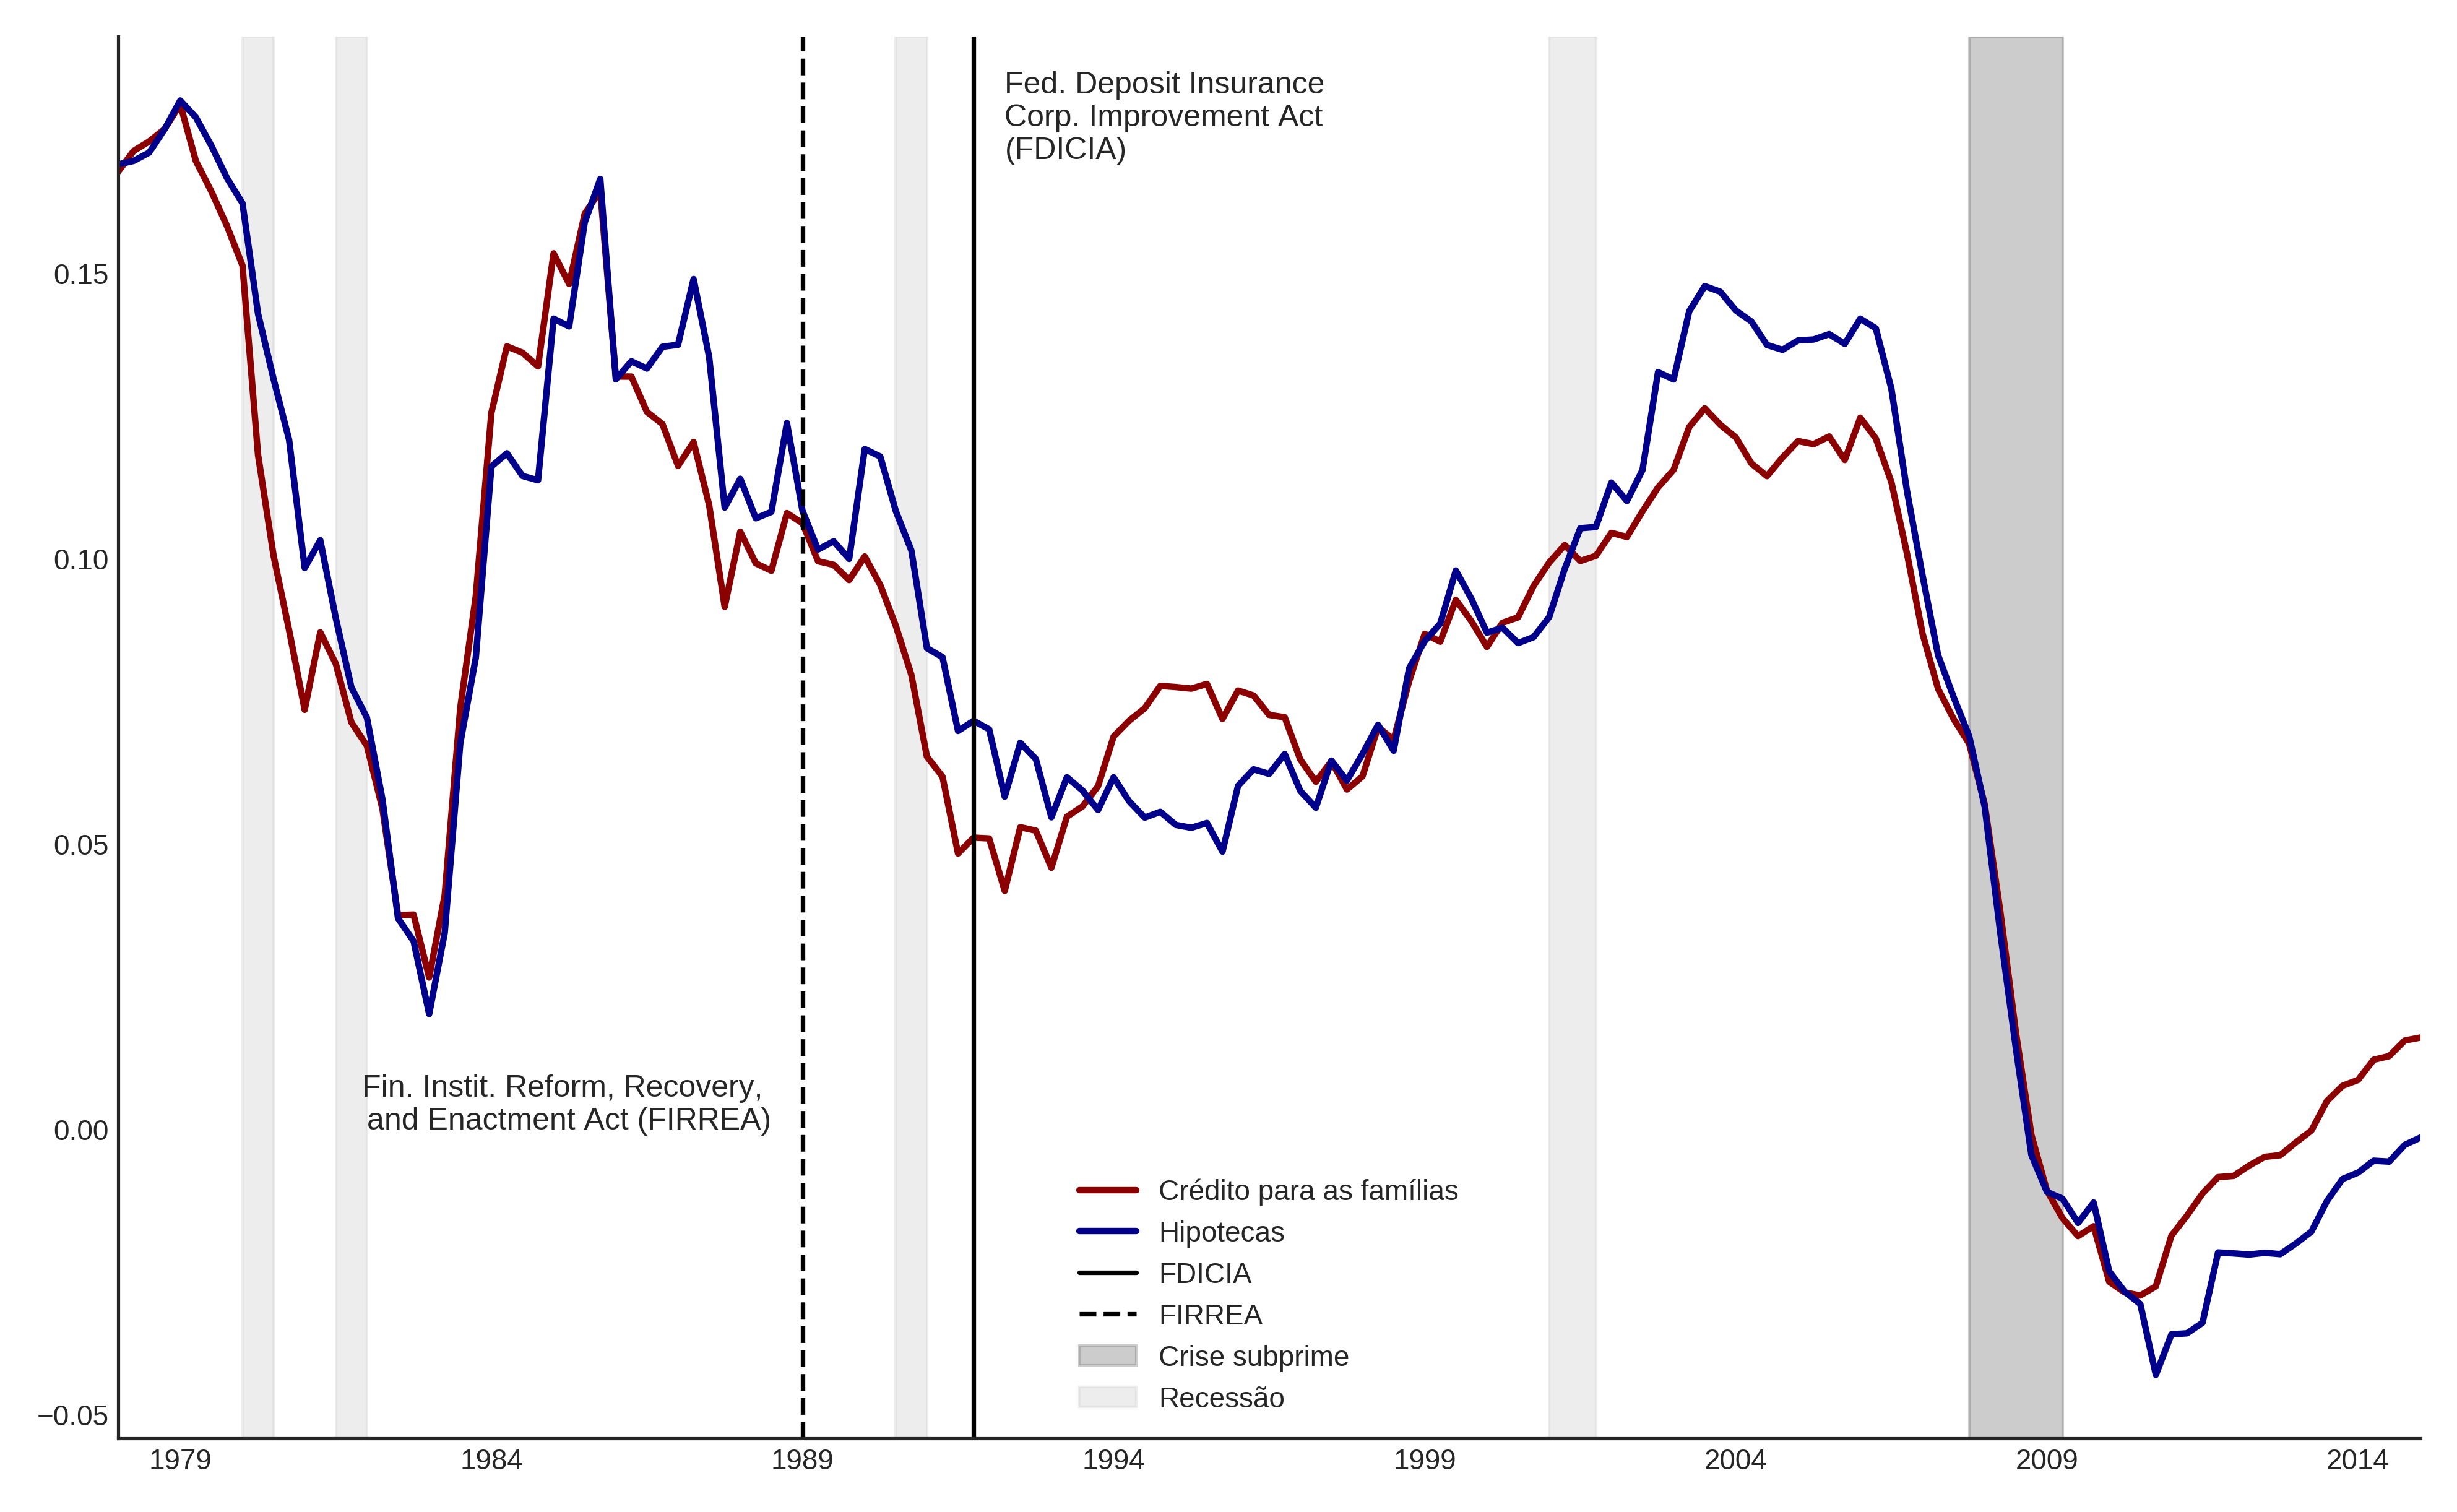
\includegraphics[width=\textwidth]{../../Dados/Fatos_Estilizados/figs/FDICIA.png}
	\caption*{\textbf{Fonte:} U.S. Bureau of Economic Analisys, elaboração própria}
\end{figure}
	
Apesar de \textcite{gauger_residential_2003} ressaltarem que a taxa de juros (de longo prazo) continua sendo relevante para explicar o investimento residencial, conclui-se que o procedimento destes autores não é o mais adequado por tratarem os juros como endógeno e determinado por agregados monetários. Sendo assim, ao seguir tal proposta incorre-se em uma inconsistência com a teoria macroeconômica contemporânea --- seja ela ortodoxa ou heterodoxa --- de que a taxa de juros é uma variável exógena determinada por meio de um processo decisório pela autoridade monetária de modo que a oferta de moeda é endógena \cite[p.~230--256]{lavoie_post-keynesian_2015}.

Uma forma de incluir o investimento residencial na macroeconomia da demanda efetiva sem incorrer nestes problemas é a da já mencionada taxa própria de juros dos imóveis desenvolvida por \textcite{teixeira_crescimento_2015}. A partir deste constructo teórico, é possível explicitar o custo real para se construir imóveis em termos de imóveis de modo a captar tanto o custo do endividamento quanto ganhos de capital.
Dada a compatibilidade desta especificação do investimento residencial com o supermultiplicador sraffiano, cabe a seção seguinte verificar a capacidade explicativa desta alternativa.

%ESTES ESTUDOS INDICAM A RELEVÂNCIA DO INVESTIMENTO RESIDENCIAL PARA A DINÂMICA.


\begin{comment}
No entanto, dado o objeto desta pesquisa, destaca-se aqueles trabalhos que enfatizam a importância da construção de novos imóveis para o ciclo econômico para além da contribuição de \textcite{leamer_housing_2007}.

 

\end{comment}